% !TEX root = ../notes_template.tex
\chapter{Intro to Reflexes, Pulses \& RUSI}\label{chp:reflex_pulse}

\section*{Objectives}

By the end of this week’s lab, you will be able to:

\begin{itemize}
  \item Demonstrate proper technique for eliciting deep tendon reflexes (DTRs) and interpret findings using the 0–4+ grading scale.
  \item Correlate reflex findings with segmental innervation and Week 1 muscle testing results.
  \item Identify the “5 Ps” of ultrasound scanning and demonstrate basic probe handling techniques.
  \item Distinguish echogenic properties of soft tissues and recognize common musculoskeletal ultrasound signatures.
  \item Acquire and interpret basic B-mode ultrasound images of the patellar tendon and long head of the biceps.
  \item Compare palpated pulses with corresponding ultrasound imaging to assess vascular anatomy and perfusion.
\end{itemize}

\section*{Overview}
This week focuses on examining segmental neurology and vascular supply through deep tendon reflexes (DTR), pulse palpation, and rehabilitation ultrasound imaging. These tools build upon Week 1’s muscle testing by offering complementary insights into motor output, neurovascular status, and muscle activation.

\section*{Deep Tendon Reflex Testing (DTR)}

\subsection*{Purpose and Segmental Relevance}

Deep tendon reflexes (DTRs) provide a rapid screen of the integrity of the spinal reflex arc and can support localization of neurological findings. When interpreted alongside MMT, they offer insight into the potential cause of muscle weakness. A \textbf{diminished or absent reflex} may suggest lower motor neuron (LMN) involvement, such as dysfunction at the nerve root or peripheral nerve. In contrast, an \textbf{exaggerated or brisk reflex} may indicate upper motor neuron (UMN) involvement, typically reflecting central nervous system dysfunction above the spinal reflex level.

This week, you will assess two reflexes that correspond to previously tested muscles:

\begin{itemize}
  \item \textbf{Biceps Reflex}
  \begin{itemize}
    \item \textbf{Nerve Roots:} C5–C6
    \item \textbf{Peripheral Nerve:} Musculocutaneous
  \end{itemize}

  \item \textbf{Patellar Reflex}
  \begin{itemize}
    \item \textbf{Nerve Roots:} L3–L4
    \item \textbf{Peripheral Nerve:} Femoral
  \end{itemize}
\end{itemize}

\subsection*{General Guidelines for Reflex Testing}

Effective reflex testing requires both proper setup and refined technique. Follow these guidelines to elicit accurate and interpretable responses:

\begin{itemize}
  \item \textbf{Position the patient:} The limb being tested should be relaxed and partially supported. Use a gravity-neutral position when possible.
  \item \textbf{Identify the tendon:} Palpate and locate the tendon to be tapped. If needed, slightly stretch the tendon to increase responsiveness.
  \item \textbf{Stabilize the segment:} Use your non-dominant hand to support or stabilize the proximal joint without tension.
  \item \textbf{Use a quick wrist motion:} Tap the tendon briskly with a reflex hammer, using a relaxed wrist and smooth follow-through.
  \item \textbf{Observe the response:} Look for the muscle’s immediate contraction—not just limb movement. Repeat 2–3 times if needed.
  \item \textbf{Compare bilaterally:} Always test both sides to assess symmetry and establish a functional baseline.
\end{itemize}

\subsection*{Grading and Interpretation}

Reflexes are graded on a standardized 0–4+ scale:

\begin{itemize}
  \item \textbf{0:} Absent (areflexia)
  \item \textbf{1+:} Diminished (hyporeflexia)
  \item \textbf{2+:} Normal
  \item \textbf{3+:} Brisk (may be normal or early hyperreflexia)
  \item \textbf{4+:} Clonus (sustained reflex activity; pathological)
\end{itemize}

\textit{Interpretation Tip:} A reduced or absent reflex may indicate a peripheral or lower motor neuron lesion. A brisk or exaggerated reflex may point toward an upper motor neuron lesion.

\begin{labactivitybox}
\textbf{Activity: Segmental Reflex Screening – Biceps and Patellar}

Perform and grade the biceps and patellar reflexes on both limbs. Use your Week 1 MMT findings to inform your interpretation.

\textit{Record:}
\begin{itemize}
  \item Reflex grade (0–4+) for each limb.
  \item Is the response symmetrical?
  \item Does the reflex correlate with your MMT findings?
  \item What would a hypo- or hyper-reflexive finding suggest?
\end{itemize}
\end{labactivitybox}

\section*{Introduction to Rehabilitative Ultrasound Imaging (RUSI)}

Rehabilitative Ultrasound Imaging (RUSI) allows real-time visualization of soft tissue structures to support functional assessment and therapeutic reasoning. Unlike diagnostic imaging, which aims to detect pathology, RUSI augments a physical therapist’s clinical reasoning by enabling observation of muscle contraction, tendon morphology, fascial continuity, and spatial relationships during clinical tasks and dynamic movement.\footnote{Conceptual framework adapted from Teyhen et al. (2007), \textit{Rehabilitative Ultrasound Imaging}; technical notes adapted from Coppola, S. DPT (2024), \textit{Diagnostic Ultrasound Notes}.}

\section*{Introduction to Rehabilitative Ultrasound Imaging (RUSI)}

Rehabilitative Ultrasound Imaging (RUSI) allows real-time visualization of soft tissue structures to support functional assessment and therapeutic reasoning. Unlike diagnostic ultrasound imaging, which aims to detect pathology, RUSI augments a physical therapist’s clinical reasoning by enabling observation of muscle contraction, tendon morphology, fascial continuity, and spatial relationships during clinical tasks and dynamic movement.\footnote{Conceptual framework adapted from Teyhen et al. (2007), \textit{Rehabilitative Ultrasound Imaging}; technical notes adapted from Coppola, S. DPT (2024), \textit{Diagnostic Ultrasound Notes}.}

\subsection*{Fundamentals of Ultrasound Imaging}

\begin{itemize}
  \item \textbf{Probe Type:} We will mostly use a \textbf{linear transducer} (7–15 MHz) optimal for superficial musculoskeletal structures.

  \item \textbf{Probe Orientation:} 
  \begin{itemize}
    \item \textbf{Long Axis (LAX):} Indicator toward head — left side of screen is cephalad.
    \item \textbf{Short Axis (SAX):} Indicator to patient’s right — left side of screen is lateral.
  \end{itemize}

  When the probe is held perpendicular to the surface, the ultrasound machine generates a real-time “slice” of the anatomy immediately beneath it. In \textbf{Long Axis (LAX)}, the image represents a longitudinal view—like looking along the length of a muscle or tendon. In \textbf{Short Axis (SAX)}, the image is a transverse cross-section of the structures. The structures seen on screen represent only that specific 2D imaging plane under the probe.

  \item \textbf{Image Modes:} B-mode (brightness mode) creates grayscale cross-sectional images from echo amplitudes.

  \item \textbf{Key Settings:} 
  \begin{itemize}
    \item \textbf{Depth} — adjust to position of target structure.
    \item \textbf{Gain} — controls brightness uniformly.
    \item \textbf{TGC} (Time Gain Compensation) — adjusts brightness at different depths.
  \end{itemize}
\end{itemize}

\begin{figure}[H]
\centering
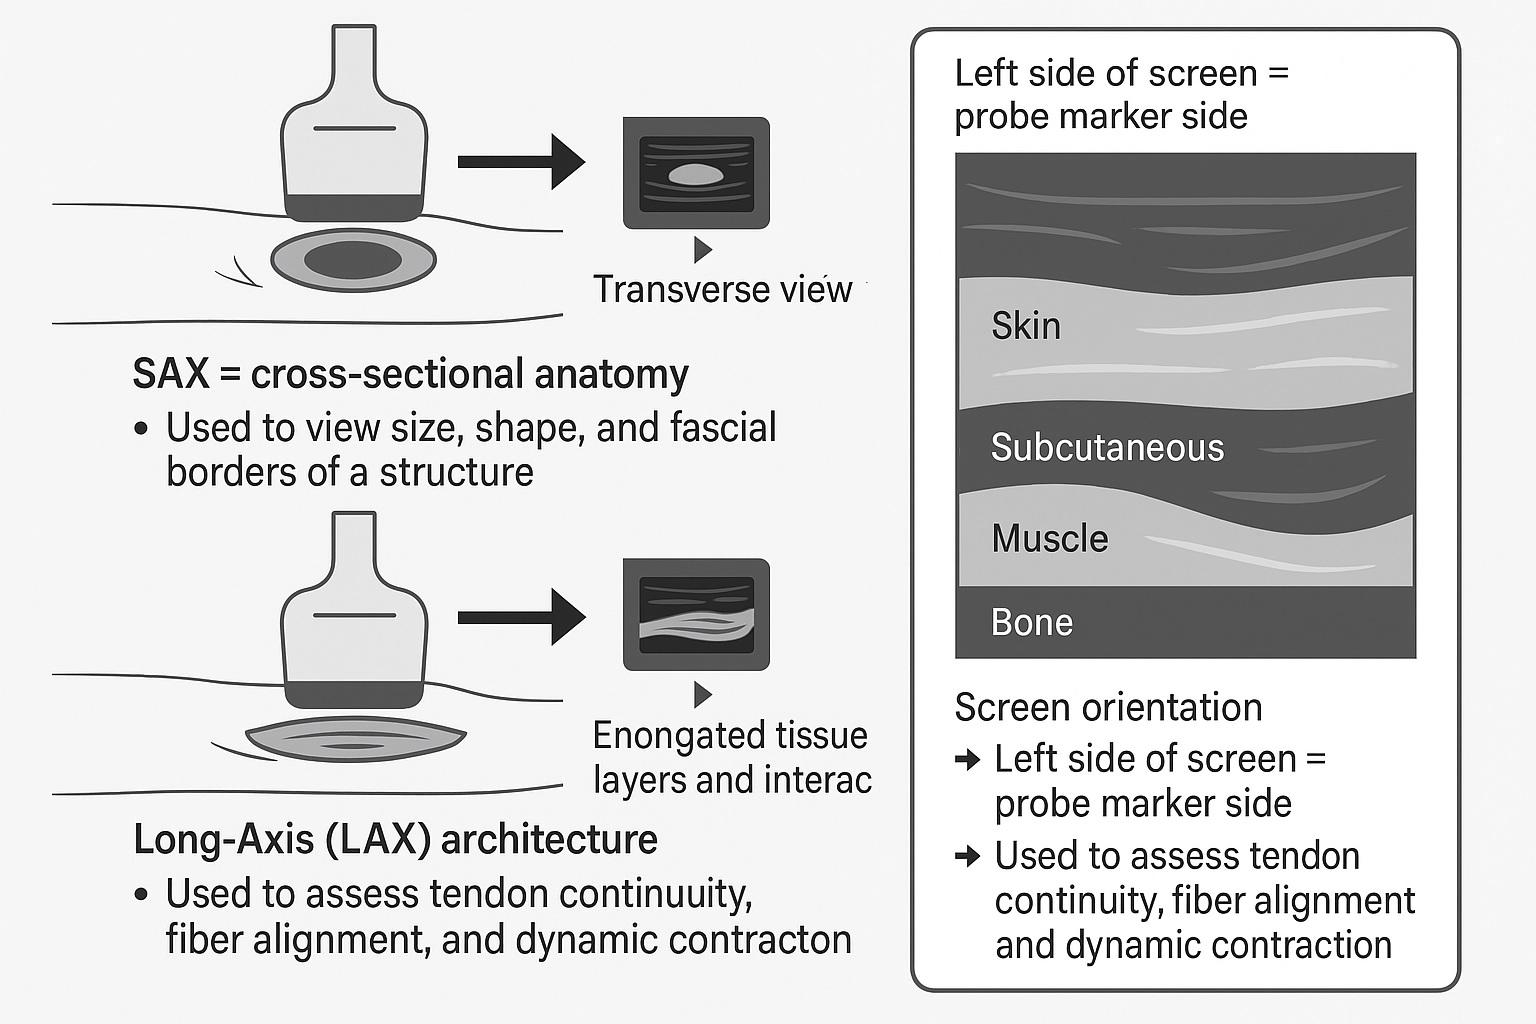
\includegraphics[width=0.75\textwidth]{figure/ultrasound_probe_orientation.png}
\caption{Schematic visualization of ultrasound probe placement: Short-Axis (SAX) and Long-Axis (LAX) views. Arrows indicate the path of the sound beam and screen orientation. This convention is foundational for interpreting RUSI scans across multiple anatomical regions.}
\label{fig:probe_orientation}
\end{figure}

\subsection*{Understanding Echogenicity}

Echogenicity refers to the ability of a tissue to reflect ultrasound waves and appear on the screen as varying shades of brightness:

\begin{itemize}
  \item \textbf{Hyperechoic:} Tissues that reflect many sound waves, appearing bright or white (e.g., bone, tendon).
  \item \textbf{Hypoechoic:} Tissues that reflect fewer sound waves, appearing darker gray (e.g., muscle).
  \item \textbf{Anechoic:} Structures that do not reflect sound waves, appearing completely black (e.g., blood-filled vessels).
\end{itemize}

\subsection*{Tissue Signatures on Ultrasound}

\begin{itemize}
  \item \textbf{Muscle (LAX):} Feather-like hypoechoic bundles with hyperechoic septa.
  \item \textbf{Tendon (LAX):} Bright, fibrous, striated appearance; more echogenic than muscle.
  \item \textbf{Nerve (SAX):} “Honeycomb” pattern — hypoechoic fascicles with hyperechoic boundaries.
  \item \textbf{Bone:} Continuous hyperechoic line with posterior shadowing.
  \item \textbf{Vessels:} Anechoic circles; arteries are pulsatile and non-compressible, veins compress with pressure.
\end{itemize}

\subsection*{Anisotropy}

Anisotropy refers to the angle-dependent appearance of certain tissues on ultrasound—particularly tendons and nerves. These structures are highly reflective when the sound waves strike them at a perpendicular angle. If the probe is slightly tilted (not perpendicular), the returning echoes are diminished, and the structure appears falsely dark (hypoechoic).

\textbf{Clinical Implication:} A healthy tendon may appear pathologically dark if scanned at a poor angle. To correct for anisotropy, use heel-toe adjustments or fine probe tilting to maintain a perpendicular beam. This technique is especially important when imaging linear structures like the patellar tendon or long head of biceps.

\subsection*{The 5 Ps of Ultrasound Scanning}

To support consistent scanning performance, this lab uses the “5 Ps” framework developed by Coppola, S. DPT (2024):\footnote{Adapted from Coppola, S. DPT (2024), \textit{Diagnostic Ultrasound Notes}.}

\begin{itemize}
  \item \textbf{Patient Position:} Ensure the patient is relaxed and optimally positioned for the target region.
  \item \textbf{Provider Position:} Position yourself ergonomically, with stable posture and clear visualization of the screen.
  \item \textbf{Probe Position:} Align the probe with appropriate orientation (LAX or SAX), contact, and angle relative to the anatomy.
  \item \textbf{Parameters:} Adjust depth, gain, and TGC for optimal visualization of the target structure.
  \item \textbf{Picture:} Evaluate the image for clarity, contrast, and correct anatomical relationships.
\end{itemize}

\subsection*{Operational Techniques}

\begin{itemize}
  \item \textbf{Static Scanning:} Position the probe using a known bony window, minimize motion, adjust image.
  \item \textbf{Dynamic Scanning:} Incorporate movement or muscle contraction; stabilize probe and observe response.
  \item \textbf{Techniques:} Fanning, heel-toe, rotating, sliding (translation) — performed slowly with controlled pressure.
\end{itemize}

\subsection*{Describing Probe Motion Techniques}

The following probe maneuvers help optimize image clarity, alignment, and depth of field:

\begin{itemize}
  \item \textbf{Heel-Toe:} Tilting the probe on its long axis to angle the ultrasound beam inferiorly or superiorly without translation.
  \item \textbf{Fanning:} Pivoting the probe across a fixed point to scan through a structure in sequential planes (like tilting on its short axis).
  \item \textbf{Sliding (Translation):} Moving the entire probe across the skin while maintaining orientation.
  \item \textbf{Rotation:} Turning the probe about its axis to switch between long and short axis views.
\end{itemize}

\begin{figure}[H]
  \centering
  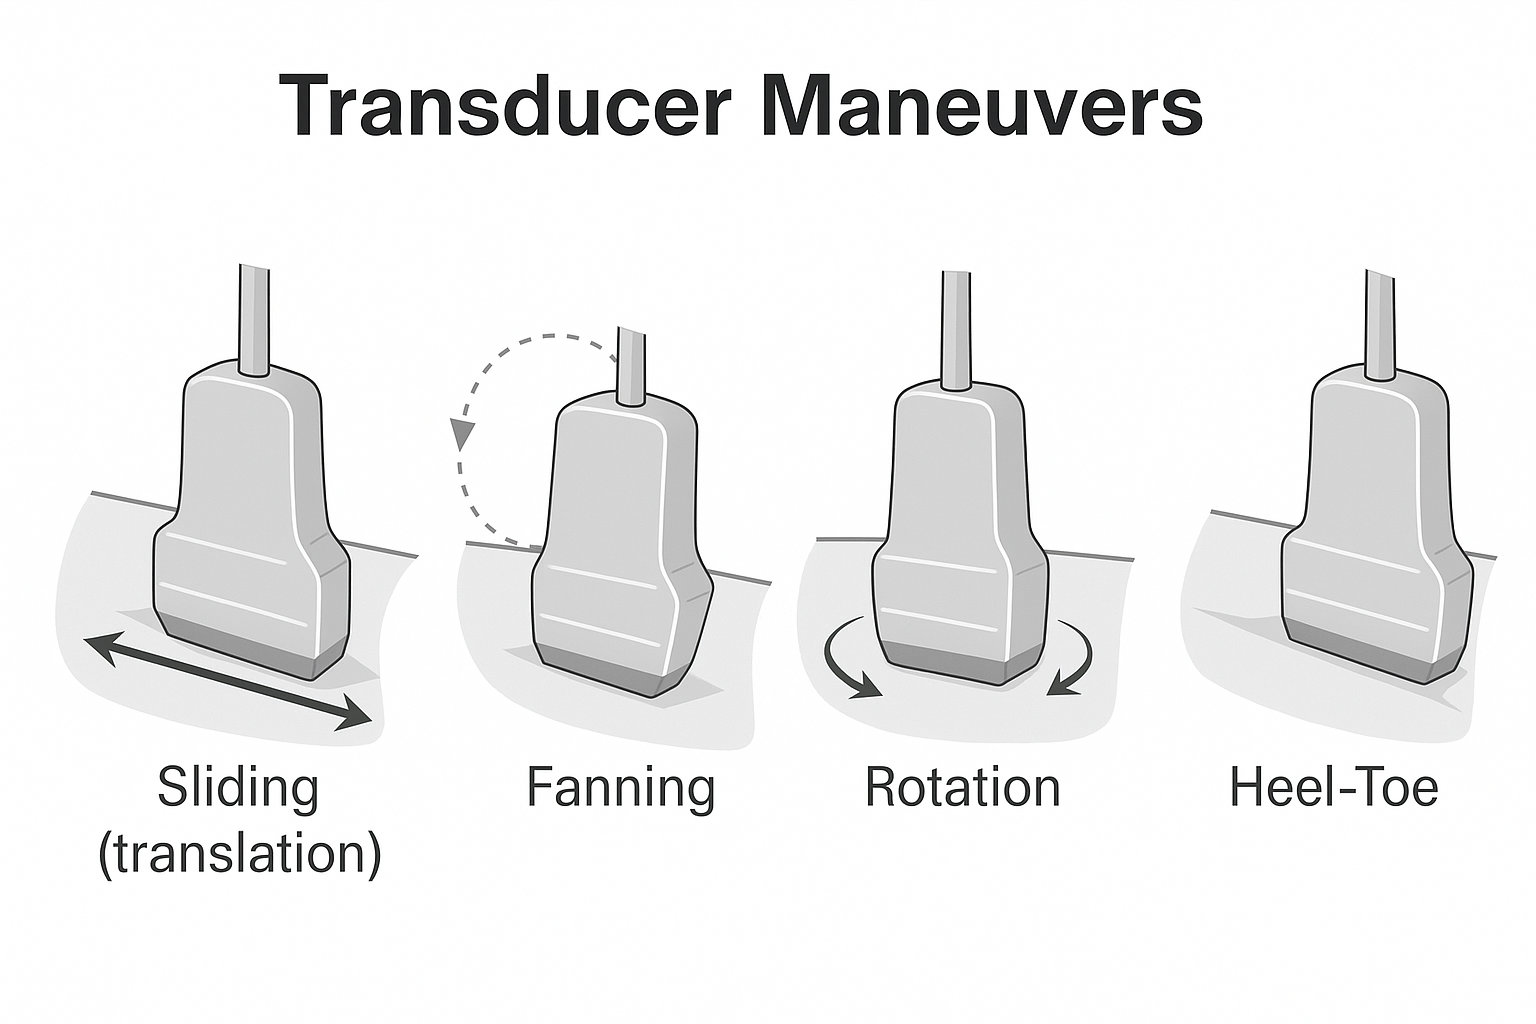
\includegraphics[width=0.6\textwidth]{figure/transducer_manuevers.png}
  \caption{Transducer manipulation techniques: Heel-Toe, Fanning, Sliding, and Rotation. Adjustments like these are essential for image clarity, anatomical accuracy, and resolving anisotropy.}
  \label{fig:transducer_maneuvers}
\end{figure}

\subsection*{Clinical Relevance in this Lab}

RUSI will be used:
\begin{itemize}
  \item To observe superficial muscle morphology (e.g., thickness, contraction, and symmetry).
  \item To assess dynamic muscle motion during voluntary contraction or positioning.
  \item To visualize vascular structures and assess pulse presence, especially when distal perfusion is in question.
\end{itemize}

\textbf{Integration Note:} As you learn RUSI, connect image interpretation with your anatomical palpation, movement analysis, and neural tracing skills. This is not an isolated tool—it is a window into functional anatomy in motion.

\medskip

\subsection*{RUSI Lab Activities}

\begin{labactivitybox}
\textbf{Activity: RUSI Session 1 – Patellar Tendon}

Use a linear transducer to visualize the patellar tendon in long axis (LAX) and short axis (SAX). This session emphasizes probe alignment, depth adjustment, and recognition of anisotropy.

\textit{Steps:}
\begin{enumerate}
  \item Position the patient supine with the knee extended.
  \item Palpate the patellar tendon between the inferior pole of the patella and tibial tuberosity.
  \item Place the probe in LAX and adjust depth and gain for optimal visualization.
  \item Identify the bright linear structure of the tendon and underlying hyperechoic bone with shadowing.
  \item Rotate to SAX view and confirm the round, fibrous tendon appearance.
\end{enumerate}

\textit{Record:}
\begin{itemize}
  \item Which transducer orientation yielded the clearest image of tendon structure?
  \item Was anisotropy present? How did you resolve it?
  \item What adjacent structures were visible in each view?
\end{itemize}
\end{labactivitybox}

\vspace{1em}

\begin{labactivitybox}
\textbf{Activity: RUSI Session 2 – Biceps Tendon (Long Head)}

This scan focuses on the long head of the biceps tendon in the bicipital groove, introducing layered anatomy, bony landmarks, and SAX vs. LAX confirmation.

\textit{Steps:}
\begin{enumerate}
  \item Position the patient seated with arm resting and slightly externally rotated.
  \item Identify the bicipital groove just distal to the acromion.
  \item Begin with SAX view: the tendon should appear as a bright oval structure between two bony ridges.
  \item Rotate to LAX to view the longitudinal path of the tendon toward the musculotendinous junction.
  \item Adjust for anisotropy, gain, and depth as needed.
\end{enumerate}

\textit{Record:}
\begin{itemize}
  \item How did the bony landmarks help guide your probe orientation?
  \item Which artifacts were present, and how were they addressed?
  \item How does this imaging reinforce your palpation and anatomical understanding from Week 1?
\end{itemize}
\end{labactivitybox}

\section*{Pulse Palpation}

\subsection*{Clinical Significance of Pulse Palpation in Muscle Assessment}

Palpating a peripheral pulse is not only about identifying cardiovascular health; it also serves as an essential screen of local muscle perfusion. Muscle contraction and endurance rely on sufficient delivery of oxygen and nutrients through the extracellular fluid (ECF), and adequate removal of metabolic byproducts. These principles are foundational to skeletal muscle physiology and become especially relevant in cases of weakness, fatigue, or inflammation.

The capillary microcirculation within muscle is supported by systemic and regional arterial flow, and even subtle limitations in perfusion can compromise muscle performance. Thus, assessing pulse strength and symmetry provides valuable insight into possible vascular or autonomic contributions to impaired muscle function.

Ultrasound can augment this assessment by directly visualizing arterial pulsatility and compressibility in real time, reinforcing what is palpated with the hands. \footnote{Adapted from Chapters 7 and 9 of \textit{Clinical Physiology: A Muscle-Centered Approach}}

\subsection*{Palpation Augmented by Ultrasound}

Palpation of peripheral pulses is a foundational skill in assessing circulation, perfusion, and vascular integrity. While clinical practice typically relies on tactile pulse grading, ultrasound can augment this process by directly visualizing arterial pulsatility and vessel compressibility.

In this lab, you will combine manual pulse palpation with B-mode ultrasound to enhance your understanding of vascular location, depth, and response.

\textbf{Target Pulse: Radial Artery}
\begin{itemize}
  \item Located just lateral to the flexor carpi radialis tendon at the distal forearm.
  \item Best visualized in short axis with the probe placed transversely over the artery.
  \item Appears as a round, anechoic vessel; observe wall motion or use light pressure to confirm pulsatility.
\end{itemize}

\begin{labactivitybox}
\textbf{Activity: Palpating and Imaging the Radial Pulse}

\textit{Steps:}
\begin{enumerate}
  \item Palpate the radial pulse using light finger pressure on both wrists.
  \item Grade the strength of the pulse on a 0–4+ scale.
  \item Place the linear transducer transversely over the palpated site and visualize the artery.
  \item Observe real-time pulsatility and compare symmetry between sides.
  \item Apply gentle compression to assess vessel compressibility.
\end{enumerate}

\textit{Record:}
\begin{itemize}
  \item Pulse strength (0–4+) and symmetry by palpation.
  \item Was the artery visible on ultrasound? What settings or adjustments improved the image?
  \item Did ultrasound confirm your palpation findings?
  \item What was the relationship between probe angle, compression, and arterial visualization?
\end{itemize}
\end{labactivitybox}

\section*{Clinical Integration}

This week’s lab expanded the diagnostic value of manual testing by integrating reflexes, vascular assessment, and imaging. Deep tendon reflexes help clarify whether muscle weakness stems from lower motor neuron (LMN) involvement (reduced reflexes) or possible upper motor neuron (UMN) involvement (brisk or clonic reflexes). When paired with MMT, reflex findings provide additional insight into whether reduced strength may have a neural origin.

Rehabilitative ultrasound imaging (RUSI) confirmed muscle presence, morphology, and contraction symmetry—adding visual validation to your palpation and manual testing findings. Pulse palpation, augmented by imaging, emphasized the critical role of local perfusion in muscle function and endurance. Together, these tools reinforce a systems-based view of neuromuscular performance.

\section*{Next Steps}

\begin{itemize}
  \item Continue practicing reflex testing using proper positioning and grading scales.
  \item Review and reinforce the nerve root–muscle–reflex mapping introduced in Weeks 1–2.
  \item Practice RUSI techniques during open lab hours: probe stabilization, depth/gain settings, and tissue recognition.
  \item Begin previewing the upper extremity regional testing approach for Week 3, especially MMT and MLT of the shoulder girdle.
\end{itemize}

\section*{Checklist Summary}

\begin{itemize}
  \item [$\square$] Performed and graded deep tendon reflexes (DTRs) for biceps and patellar tendons, using the 0–4+ scale.
  \item [$\square$] Interpreted DTR findings in relation to muscle weakness and motor neuron involvement.
  \item [$\square$] Identified musculoskeletal tissue types (muscle, tendon, nerve, bone, vessel) on ultrasound using proper LAX and SAX orientation.
  \item [$\square$] Applied the “5 Ps” of scanning and demonstrated effective use of probe motion techniques (heel-toe, fanning, sliding, rotation).
  \item [$\square$] Acquired and interpreted B-mode ultrasound images of the patellar and biceps tendons in both LAX and SAX views.
  \item [$\square$] Visualized and confirmed the radial artery using ultrasound, assessing pulsatility and compressibility.
  \item [$\square$] Compared palpated radial pulse with ultrasound visualization, noting symmetry and vessel location.
\end{itemize}

